\documentclass[11pt]{article}
\usepackage[margin=1in]{geometry}
\usepackage{pdfpages}
\usepackage[sfdefault]{GoSans}
\usepackage{longtable}
\usepackage{array}
\usepackage{verbatim}
\linespread{1,5}


\begin{document}
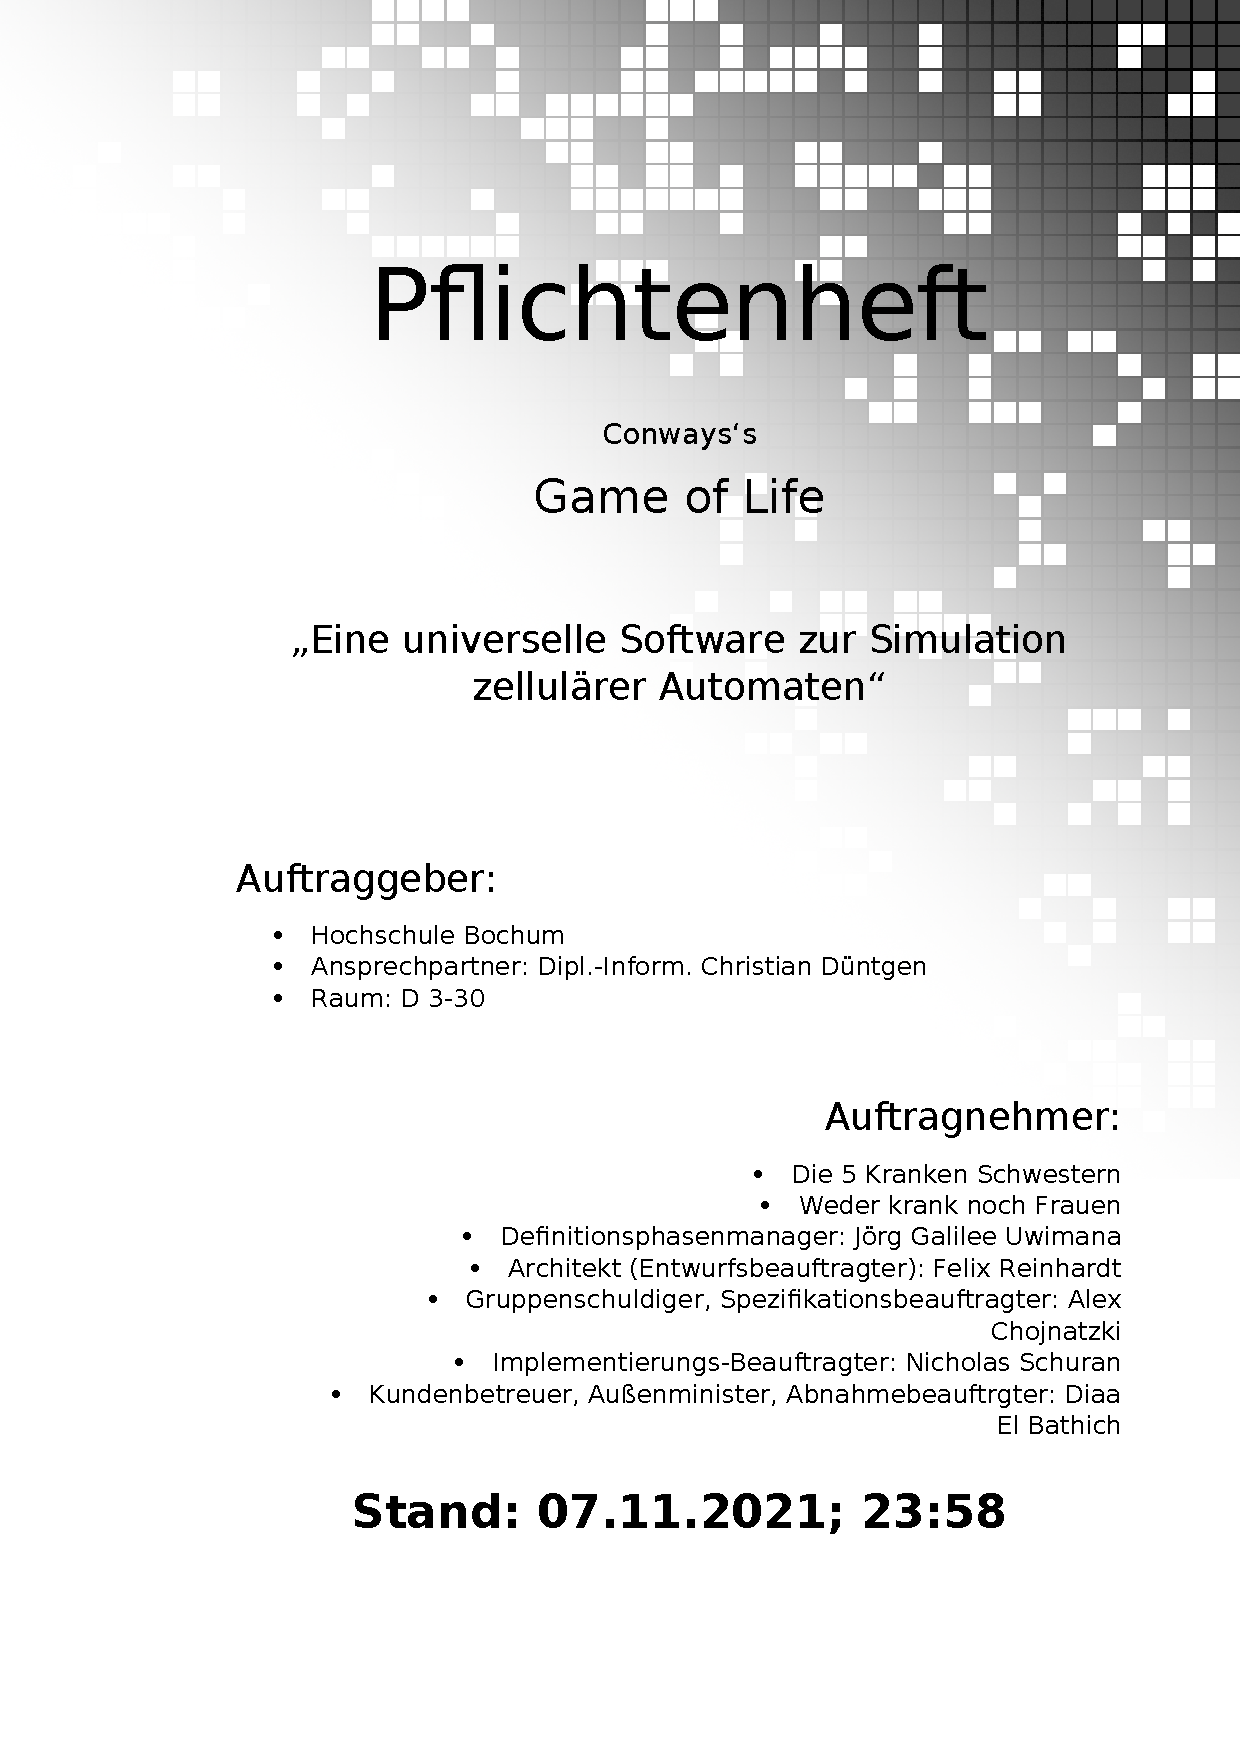
\includepdf[]{DeckblattPflichtenheft.pdf}
\title{Pflichtenheft}

\author{Die kranken Schwestern}

\tableofcontents
\pagebreak

\section{Zielbestimmung}
\subsection{Musskriterien}
Das Programm soll dazu dienen, Zelluläre Automaten auf einem 2-D orthogonalen Spielfeld darstellen zu können. Dazu werden als Beispiel die Regeln für Conway`s Game of Life verwendet.
Hierzu sind unbedingt die folgenden Features erforderlich:

\par



\begin{longtable}[m]{|m{2.2cm}|m{4cm}|m{8cm}|}
\hline
M0001     & UI & Das Programm muss eine graphische Oberfläche haben.  \\
\hline
M0002 & Scope & •	Es soll ein zellulärer Automat mit möglichst großer Freiheit definiert und simuliert werden können.  \\
\hline
M0003 & Darstellung Spielfeld & •	Die Darstellung des Zellulären Automaten erfolgt über eine 2 Dimensionale Matrix aus Quadraten deren Farbe und Helligkeit den Zustand eines Feldes wiedergeben. \\
\hline
M0004 & Transitionsregeleditor & Die Transitionsregeln sollen über eine definierte und im Handbuch dokumentierte Syntax (invers Polnische Notation, ggf. auch mathematische Schreibweise) formuliert werden können. Der neue Zustand einer Zelle darf dabei von der Zelle selbst, sowie von den umliegenden acht benachbarten Zellen abhängen. Ihr Status wird in Variablen bereitgestellt.\\
\hline
M0005 & Spielfeldaufbau & Das Spielfeld soll als 2-D Array von Integerwerten ausgeführt sein, welche den Zellzustand repräsentieren.\\
\hline
0006 & Spielfeldgröße & Die Spielfeldgröße soll vor Simulationsstart vom Benutzer über (Text-)Eingabefelder festgelegt werden können.\\
\hline
M0007 & Speichern \& Laden & Spielfeldzustand und Transitionsregeln sollen seperat gespeichert und geladen werden können.  \\
\hline
M0008 & Einfügen & Es sollen Figuren in das Spielfeld eingefügt werden können. Dies soll so geschehen, dass Figuren als Spielstände mit kleinerer Feldgröße als ganzes geladen und eingefügt werden können. \\
\hline
M0009 & Navigation & es soll möglich sein, das Spielfeld mit Zoom und Pan verschieden zu betrachten. \\
\hline
M0010 & Spielfeldmanipulation & Der Zustand einer Zelle soll durch Mausklick darauf auf einen wählbaren Wert einstellbar sein. Das Wählen des Werts soll durch ein Texteingabefeld auf der Benutzeroberfläche erfolgen. Details in der Beschreibung der Benutzeroberfläche.\\
\hline
M0011 & Topologie & Das Randverhalten des Spielfelds soll zwischen begrenztem Rechteck und Torus (Zellen an den Kanten sind mit den ihnen gegenüberliegen zellen benachbart) wählbar sein.\\
\hline
M0012 & Automatische Simulation & Die Simulationsgeschwindigkeit soll über einen Slider einstellbar sein. Die Simulation soll über einen Button gestartet und unterbrochen werden können.\\
\hline
M0013 & Manuelle Simulation & Über einen Button soll die nächste Generation berechnet und angezeigt werden können. \\
\hline
M0013 & Zufälliger Anfangszustand & Der Spielfeldzustand soll zufällig generierbar sein. Dazu soll einem Zellzustand eine Wahrscheinlichkeit zugewiesen werden können, mit dem Default-Zustand 0, sodass jede Zelle genau einen Zustand erhält.\\

\hline
M0014 & Anzeige & Die Anzeige des Spielfeldzustands soll durch Farben erfolgen, wobe einem Zustand eine Farbe zugeordnet wird.\\
\hline
M0015 & Startbedingungen & Beim Programmstart soll ein 80x80 Zellen großes Spielfeld präsentiert werden, auf welches die Spielregeln für Conway's Game of Life verwendet werden. \\

\hline
\end{longtable}    
\newpage
\begin{comment}


\begin{itemize}
    \item Nach dem Programmstart soll dem Benutzer ein 80x80 Felder großes Spielfeld präsentiert werden. Unterhalb des Spielfeldes sind verschiedene Knöpfe und Kontrollen anzuordnen, welche im folgenden näher erläutert werden sollen.
    \item Es ist erforderlich, die Simulation zu starten und zu stoppen, hierzu wird ein Button benötigt. 
    \item Es ist erforderlich, eine einzelne Generation weiter springen zu können, dies benötigt ebenfalls einen Button.
    \item Es ist Sinnvoll, die Simulationsgeschwindigkeit einstellen zu können, dies soll in Form eines Sliders geschehen. Die Simulationsgeschwindigkeit soll zwischen 0,5 und 10 Generationen pro Sekunde frei Wählbar sein.
    \item Es soll die Größe des Spielfeldes anpassbar sein. Dies soll so geschehen, dass über einen Button auf dem Hauptinterface ein Fenster aufgerufen wird, auf dem die Größe des Spielfeldes mit zwei Eingabefeldern als int,  sowie Randverhalten eingestellt werden können.
    \item Das Randverhalten soll zwischen zwei Optionen mit RadioButtons oder ähnlichem wählbar sein, sodass das Spiel entweder auf einer endlichen Fläche mit toten Rändern läuft, oder torusartig an den Enden zusammengebogen wird.
    \item Es ist gewünscht, dass die Spielregeln anpassbar sind. Dies soll über eine Eingabezeile geschehen, welche in einem Regeleditor existiert. Der Regeleditor soll über einen Button auf dem Hauptinterface aufrufbar sein.
    \item Es ist hochgradig nützlich, einen Spielstand speichern und laden zu können. Dies soll einfach gehalten werden: es soll der Zustand des Feldes sowie der Zustand des Regeleditors in eine Datei ausgelagert werden.
    \item Zum Laden von Spielständen: Es sollen Spielstände von der Festplatte geladen werden können. Dies soll auch dazu dienen, bereits bekannte Spielfeldkonstruktionen in das aktuelle Spielfeld einzufügen. Das bedeutet, dass es ein "komposit-laden" geben soll: Wird dies ausgewählt UND ist das Spielfeld des zu ladenden Spielstands kleiner als das Aktuelle, so soll per Mausklick das zu ladende Spielfeldkonstrukt das Spielfeld an den entsprechenden Stellen überschreiben und das Konstrukt so in das Spiel integrieren.
    \item Das Spielfeld soll als zweidimensionales Array ausgeführt sein, in welchem Integer-Werte einen Zellzustand festlegen. Dieses soll im Hauptfenster angezeigt werden, wobei die verschiedenen Zellzustände durch Farben angedeutet werden sollen.
    
    
    
    
\end{itemize}

\end{comment}
\subsection{Wunschkriterien}
\begin{longtable}[m]{|m{2.2cm}|m{4cm}|m{8cm}|}
\hline
W0001 & Undo & Es sollen Eingaben rückgängig gemacht werden können.\\
\hline
W0002 & Regeleditor & Eingabe der Regeln in für Menschen gut lesbarer Mathematischer Schreibweise, mit Grundrechenarten und logischen Operationen\\
\hline
W0003 & Performance & Multithreading parallelisierbarer Prozesse\\
\hline
W0003 &Farbanpassung & Wenn möglich soll die Farbe eines Zustands durch den Benutzer einstellbar sein.\\
\hline
\end{longtable}


\pagebreak
\section{Produkt-Einsatz}
\subsection{Anwendungsbereich}
Das Programm soll dazu dienen, Zelluläre Automaten mit recht großer Freiheit bauen zu können. Ob es sich dann um Game of Life, einen Waldbrandsimulator handelt, ist dann außen vor.
\subsection{Zielgruppen}
Die Verwendung dieses Programms für Conway's Game of life ist einfach, da die Spielregeln mitgeliefert werden. Dies kann von allen interessierten ausprobiert werden, da die Manipulation des Spielfelds zum ausprobieren einlädt.

Leider ist es nicht möglich, den Regeleditor intuitiv bedienbar zu gestalten, da es für eine effiziente Verarbeitung notwendig ist, den Zustand einer Zelle in der nächsten Generation als Mathematische Funktion der Zustönde der Nachbarzellen darzustellen. Aus diesem Grund gibt es zwar einen Leitfaden, um Mathematische Funktionen mit den Umliegenden Zellen als Ausgangsdaten zu erstellen, es ist jedoch nicht einfach, dies zu tun. Deal with it.
\subsection{Produktumgebung}
\subsubsection{Softwareanforderungen}

\subsubsection{Softwareanforderungen}
\begin{itemize}
    \item Ein "Java Runtime Envrionment" der Version 1.8.x oder neuer. Ältere Versionen werden nicht getestet.
    \item Betriebssystem, was in der Lage ist, besagte JRE auszuführen. 
\end{itemize}

\subsubsection{Hardwareanforderungen}
\begin{itemize}
    \item Ein Computer aus diesem Jahrtausend mit einer Prozessorarchitektur für die eine JRE verfügbar ist. Dual-Core oder besser empfohlen, Dienstalter nicht über 1,6 Dekaden.
\end{itemize}
\subsection{Betriebsbedingungen}
\begin{itemize}
    \item Schreib- und Leserechte für die Speicherstände.
    \item verfügbarer Speicherplatz. (500 MB Festplattenspeicher großzügigerweise empfohlen)
    \item Arbeitsspeicher angepasst an die Feldgröße (128 MB sollten für die Standardkonfiguration ausreichen)
\end{itemize}

\pagebreak
\section{Produktfunktionen}
\subsection{Funktionale Anforderungen}
\subsubsection{Benutzeroberfläche}
Nach dem Start soll folgende Oberfläche als Standard auftauchen. Im folgenden werden die (numerierten) UI-Elemente erläutert.
\subsubsection{Datenverarbeitung}
\subsubsection{Datenspeicherung}
\subsection{Nichtfunktionale Anforderungen}
\subsubsection{Performance}
\begin{itemize}
    \item Lineare Laufzeit der Generationsberechnung pro Spielfeldgröße
\end{itemize}
\subsubsection{Zuverlässigkeit}
\begin{itemize}
    \item This is bleeding edge technology. Report bugs to Jehova's Witnesses, Ortsgruppe Westfalen-Lippe.
\end{itemize}

Hinweis: Für die Sicherheit des Nutzers wird nicht garantiert.
\pagebreak
\section{Testszenarien}
Alle Testszenarien werden auf die Spezifikationsphase verschoben.
\subsection{UI}
\subsection{Verarbeitung}
\subsection{Speichern}
\subsection{Performance}
\subsection {Benutzbarkeit (Schimpanse benötigt)}
\pagebreak
\section{Entwicklungsumgebung}
\subsection{Verwendete Software}
\begin{tabular}{|c|c|}
\hline
Betriebssysteme:     &  MacOS X, Windoof X, Linux X
  \\
     \hline
     Bildbearbeitung  \&  Diaagramme & 
         GIMP, Photoshop, Modelio
 \\
     \hline
     Programmierung  \& Versionierung & 
          Eclipse, 
          Eclipse Window builder,
          GIT\\
     \hline
\end{tabular}
\subsection{Verwendete Hardware}
Intelligente Frühstücksbrettchen mit abwaschbarer Benutzeroberfläche verschiedener Hubraumklassen.
\subsection{verwendete Organisation}
Haben Sie wirklich den Eindruck, dass hier irgendwas organisiert abläuft? 
Aber gut, ein Versuch: 
Wenn etwas schief geht, ist Alex schuld.
Wenn jemand Ahnung hat, dann Nico.
Wenn jemand Protokoll schreibt, dann Felix.
Wenn jemand gute Laune hat, dann Jörg.
Wenn jemand Photoshop macht, dann Diaa.

\pagebreak




\end{document}
